%%%%%%%%%%%%%%%%%%%%%%%%%%%%%%%%%%%%%%%%%%%%%%%%%%%%%%%%%%%%%%%%%%%%%%%%%%%%%%%%%%%%%%%%%%%%%%%%
%
% CSCI 1430 Written Question Template
%
% This is a LaTeX document. LaTeX is a markup language for producing documents.
% Your task is to answer the questions by filling out this document, then to
% compile this into a PDF document.
%
% TO COMPILE:
% > pdflatex thisfile.tex

% If you do not have LaTeX, your options are:
% - VSCode extension: https://marketplace.visualstudio.com/items?itemName=James-Yu.latex-workshop
% - Online Tool: https://www.overleaf.com/ - most LaTeX packages are pre-installed here (e.g., \usepackage{}).
% - Personal laptops (all common OS): http://www.latex-project.org/get/ 
%
% If you need help with LaTeX, please come to office hours.
% Or, there is plenty of help online:
% https://en.wikibooks.org/wiki/LaTeX
%
% Good luck!
% The CSCI 1430 staff
%
%%%%%%%%%%%%%%%%%%%%%%%%%%%%%%%%%%%%%%%%%%%%%%%%%%%%%%%%%%%%%%%%%%%%%%%%%%%%%%%%%%%%%%%%%%%%%%%%
%
% How to include two graphics on the same line:
% 
% \includegraphics[width=0.49\linewidth]{yourgraphic1.png}
% \includegraphics[width=0.49\linewidth]{yourgraphic2.png}
%
% How to include equations:
%
% \begin{equation}
% y = mx+c
% \end{equation}
% 
%%%%%%%%%%%%%%%%%%%%%%%%%%%%%%%%%%%%%%%%%%%%%%%%%%%%%%%%%%%%%%%%%%%%%%%%%%%%%%%%%%%%%%%%%%%%%%%%

\documentclass[10pt,twocolumn,letterpaper]{article}
 
\usepackage{cvpr}
\usepackage{times}
\usepackage{epsfig}
\usepackage{graphicx}
\usepackage{amsmath}
\usepackage{amssymb}
\usepackage{booktabs}
\usepackage{microtype}

\usepackage{float}
% From https://ctan.org/pkg/matlab-prettifier
\usepackage[numbered,framed]{matlab-prettifier}

\frenchspacing

% Include other packages here, before hyperref.

% If you comment hyperref and then uncomment it, you should delete
% egpaper.aux before re-running latex.  (Or just hit 'q' on the first latex
% run, let it finish, and you should be clear).
\usepackage[pagebackref=true,breaklinks=true,letterpaper=true,colorlinks,bookmarks=false]{hyperref}

\cvprfinalcopy
\def\cvprPaperID{****}
\def\httilde{\mbox{\tt\raisebox{-.5ex}{\symbol{126}}}}
\ifcvprfinal\pagestyle{empty}\fi

\begin{document}

%%%%%%%%% TITLE
\title{CSCI 1430 Final Project Report:\\Un(black)boxing the Black Box}

% Make this document not anonymous
\author{
    \emph{The Stakeholders}: Siddu Sitaraman, George Chemmala, Triston Roberts.\\
    \emph{TA name:} Kamyar Mirfakhraie.
    Brown University\\
}

% Siddu: Attention (subsection of Methods), Results
% George: Related Work, Focus/Corner (subsection of Methods), Results
% Triston: Intro, Technical Discussion, SRC Discussion, Conclusion
% Arjan: Acknowledgments

\maketitle
%\thispagestyle{empty}

%%%%%%%%% ABSTRACT
% \begin{abstract}
% This document is a template for your final project reports, presented in a conference-paper style. It is sightly-more complicated LaTeX, but not much more complex than the earlier project reports. 
% This document, along with your code, any supplemental material, and your 2-minute presentation, are qualitatively what determines your grade. 
% \end{abstract}



% \section{Project Report Advice [Delete This Section]}

% \begin{enumerate}
%     \item Overriding principle: show us your effort.
%     \item If you wish us to consider any aspect of your project, it should be presented here. \item Please include a problem statement, related work, your method, your results (figures! tables!), any comparison to existing techniques, and references. 
%     \item If you made something work---great! If you didn't quite make it work---tell us about the problems, why you think it didn't work, and what you would do to fix it.
%     \item Length: Approximately four pages for techical description. For social impact, no more than one page total.
%     \item Please include an appendix to the report which details what each team member contributed to the project. One paragraph max each.
%     \item Any other materials should go in an appendix.
% \end{enumerate}


%%%%%%%%% BODY TEXT
\section{Problem Statement}
How can we adopt human-based visual processing in a convolutional neural network (CNN) in order to create a model which classifies images with greater efficiency and explainability compared to that of a traditional CNN while maintaining a comparable accuracy? 

\section{Introduction}
A crucial psychological ability that enables humans to visually comprehend physical objects is that of focusing attention selectively on certain parts of those objects. It was our aim to adapt this approach to computer image classification using CNNs to mitigate two issues with traditional CNNs while maintaining a comparable accuracy. Firstly, we aim to increase the model's efficiency by utilizing only the important, informative regions of the image. This is a challenge because it requires the model to accurately identify salient regions in the image, and what constitutes a salient region arguably varies greatly across images. Secondly, we aim to increase the model's explainability through this process by gaining more control over the sub-regions the CNN processes. This is a challenge because it is also dependent on the model to accurately identify salient regions in an image which is a non-trivial task. 

In order to solve this problem, we aim to utilize two models, the first of which being a saliency-based CNN, the second of which being an attention-based CNN. The saliency-based CNN will be split into two separate cases. For the first case it will utilize a learned focus-based CNN by initializing keypoints randomly on the image, isolating regions surrounding three of these keypoints, and train to increase accuracy in keypoint detection leading to the model's increased classification accuracy. For the second case, it will utilize a corner focus-based approach by extracting regions around the three strongest detected corners, and then training for increased corner understanding leading to increased classification accuracy. For the attention-based approach, it will operate similar to a regular CNN, but while the model takes in an image we will copy the outputs at one of the earlier layers to provide small scale information and at one of the later layers for bigger picture information. These outputs will provide insight into what the model is paying attention to, and will combine this output to that of the CNN in order to pass into our dense layer. 

To these ends, by utilizing saliency-based and attention-based CNNs, we strive toward increasing efficiency and explainability in traditional CNNs while potentially maintaining a comparable accuracy. 

\section{Related Work}

Our work builds upon several key advancements in the fields of computer vision and attention mechanisms. The use of attention mechanisms in image recognition has been explored extensively in recent years. Zhao et al.~\cite{zhao2020exploringselfattentionimagerecognition} demonstrated the potential of self-attention as a fundamental building block for image recognition models, highlighting its robustness and generalization capabilities. This aligns with our use of attention mechanisms to enhance interpretability and performance in image classification tasks.

Yan et al.~\cite{10.1007/978-3-030-20351-1_62} introduced an attention-based method for melanoma recognition, emphasizing the importance of attention maps for interpretability. Similarly, our attention-based model incorporates attention maps to provide insights into the decision-making process, making the model's predictions more transparent.

The VGG-16 architecture, as proposed by Simonyan and Zisserman~\cite{simonyan2015deepconvolutionalnetworkslargescale}, serves as the foundation for our simplified CNN model. By integrating attention mechanisms into this architecture, we aim to leverage its proven effectiveness while enhancing its interpretability.

Jetley et al.~\cite{jetley2018learnpayattention} proposed an end-to-end trainable attention module for CNNs, demonstrating its ability to highlight relevant features and suppress irrelevant ones. Our work extends this idea by applying attention mechanisms to both local and global features, enabling a more comprehensive understanding of the input image.

Finally, Nourelahi et al.~\cite{nourelahi2023explainableadversariallyrobustcnns} explored the relationship between explainability, robustness, and accuracy in CNNs. Their findings underscore the importance of balancing these criteria, which is a key consideration in all of our models' designs.

In summary, our work draws inspiration from these studies to develop models that not only achieve competitive accuracy but also provide efficency and interpretability. By focusing on keypoints and incorporating attention mechanisms, we aim to enhance the explainability of our models while maintaining their performance. Our approach aligns with the growing emphasis on interpretability in machine learning, particularly in safety-critical applications where understanding model decisions is essential.

\section{Method}

\subsection{Saliency Model}
In order to make our model "focus" on areas of the image we thought of spliting our model into 2 parts: one model to find the keypoints (keypoint model), the points in the image that are thought to hold the most important information to classify the image; and one model to use the keypoints to actually classify the image (classifier model).

We had two ideas (focus and corner detection) on how to find the keypoints and implemented both ideas in two different models, keeping the classifier the same across the 2 models. The classifier classifies the image using the keypoints by extracting a square patch (of size \(\text{patch\_size}\)) around each of the keypoints and stacking them into a tensor that we can pass into a CNN. Much like how we consider an image to be a tensor when we pass it into a CNN normally. In fact, our tensor will have shape: \[\text{patch\_size} \times \text{patch\_size} \times \text{patch\_num}\]

For example, if we pass in a \(28 \times 28 \times 1\) image into keypoint model with \(\text{patch\_size} = 5\) and \(\text{num\_keypoints} = 3\) then we get an \(5 \times 5 \times 3\) tensor that we input into our classifier model.

\subsubsection{Focus-based Model}
We first used a CNN for the keypoint model section. The image goes through a CNN which outputs a tensor of size \(2 \times \text{num\_keypoints}\) this gives us a x and y coordinate on our image for each keypoint. The model then takes the x and y coordinates and uses them to extract a square patch of size \(\text{patch\_size}\) around each keypoint. The patches are then stacked into a tensor of shape \(\text{patch\_size} \times \text{patch\_size} \times \text{num\_keypoints}\) which is passed into the classifier After we get a classification from the classifier we use the loss function to calculate the loss between the classification and the true label. We then run backpropagation through the model to update the weights of classifier and also the weights of the CNN that outputs the keypoints. Care had to be taken in order to make sure that the gradients can be backpropogated through the keypoint model since it is not trivial to make patch extraction differentiable. 

\subsubsection{Corner-based Model}
We wondered whether we could use a corner detection algorithm to find the keypoints instead of a CNN. This would probably not be as accurate as a CNN but it would be much faster in both run time and training time since we would not have to run backpropagation. We used the Harris corner detection algorithm to find the keypoints. The Harris corner detection algorithm outputs a set of corners and we select the top \(\text{num\_keypoints}\) corners. We then use the same classifier model as before to classify the image. The classifier model is the same as the one used in the focus-based model. The only difference is that we do not have to run backpropagation through the keypoint model since it is not a CNN. 

\subsection{Attention-based Model}
Attention is a technique introduced in the LLM/NLP literature that is on the cutting-edge in decision-making and generative language models. This technique allows a model to dynamically weight parts of its input while generating an output.

In this work, we sought to use attention to enhance a image-classifying CNN by having it focus on different parts of an image. We based our attention-based CNN on the model presented in Yan et al.~\cite{10.1007/978-3-030-20351-1_62}. This model extracts important intermediate layers from different depths of a CNN and interpolates them to create an attention map. We incorporate this attention map into the final dense layers of the model so that they are factored into the classification.
\begin{figure}[hbt!]
    \centering
    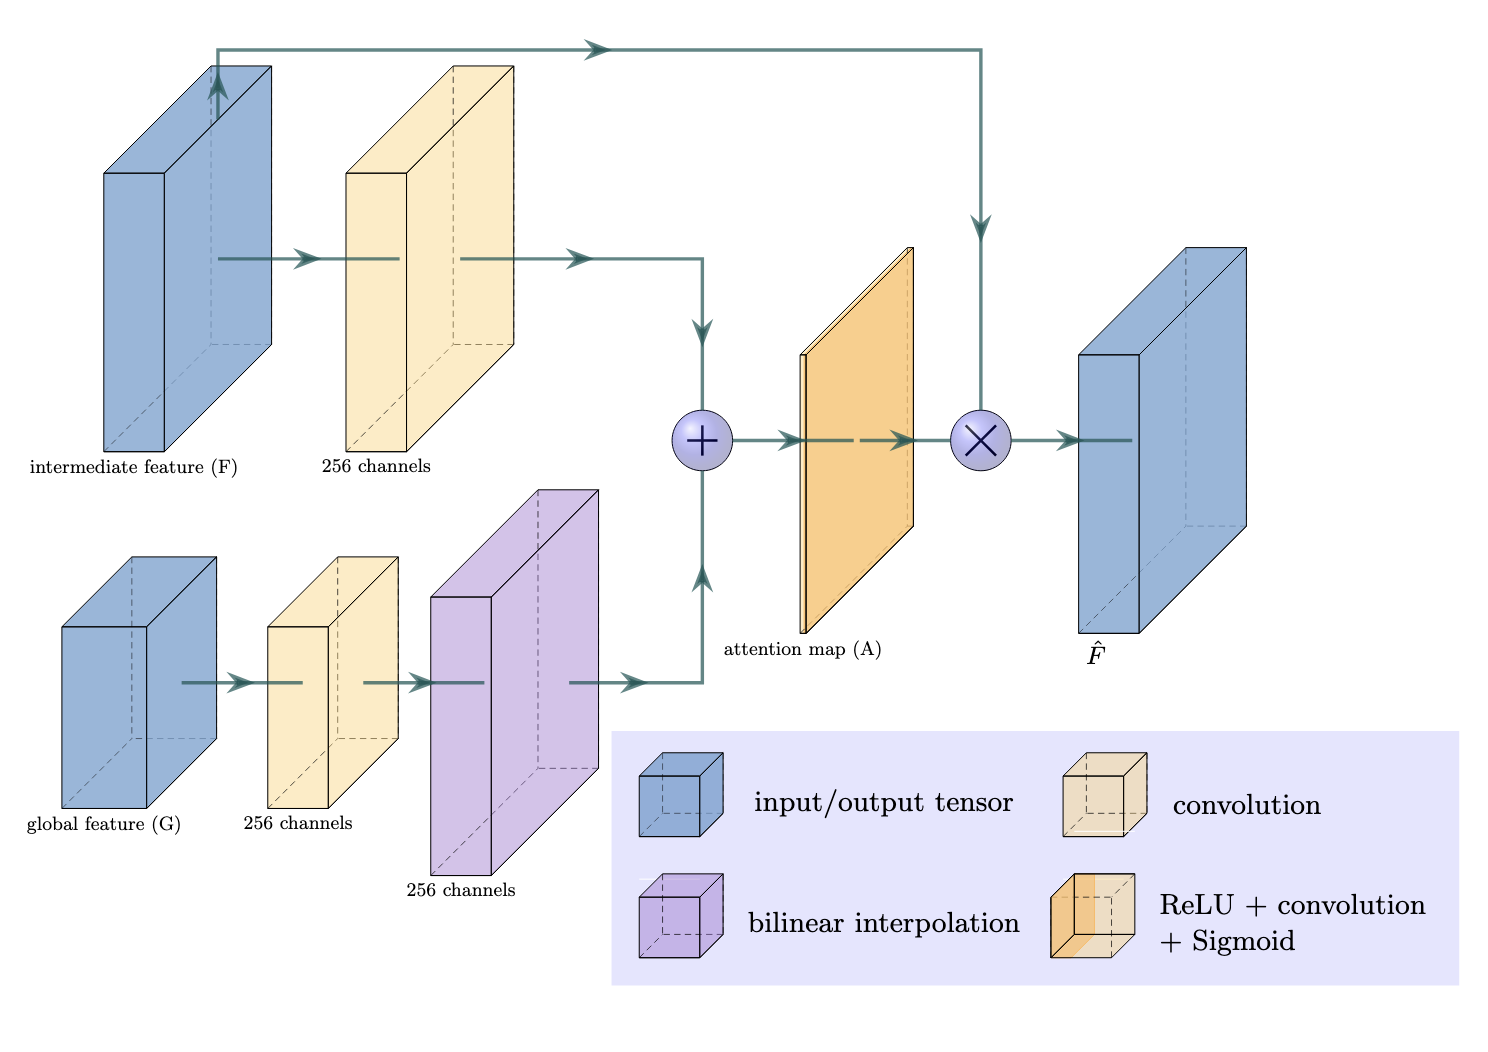
\includegraphics[width=\linewidth]{images/attentionhead.png}
    \caption{Attention block mechanics}
    \label{fig:result1}
\end{figure}

Our model uses a simplified version of the VGG-16 architecture which consists of convolutional layers followed by a neural net "head". Our construction additionally extracts a "local" layer (i.e. earlier layer) and "global" layer (i.e. later layer) and applies an attention block to them. The output of this attention block is passed through the neural network "head" for classification. 

\section{Results}
\subsection{Focus-based model results:}
The focus-based model was able to achieve a test accuracy of 98\% on the MNIST dataset using \(\text{patch\_size} = 5\). Which is comparable to the accuracy of a standard CNN. The model was able to achieve this accuracy with a much smaller number of parameters than a standard CNN.

\begin{figure}[hbt!]
    \centering
    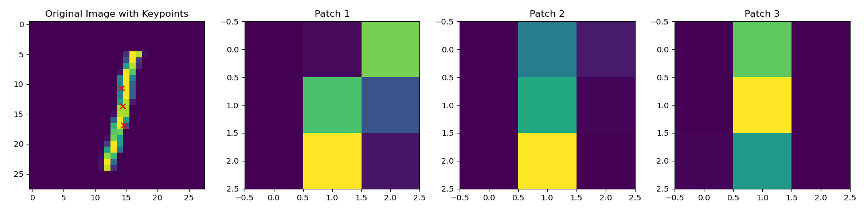
\includegraphics[scale=0.35]{images/Picture1.png}
    \caption{Here we can see that the focus-based model picked keypoints that run across the 1. This is a good example of model interpretability since we can see exactly what the model is focusing on and we can guess that the model is focusing on the straightness of the 1.}
    \label{fig:focus-1}
\end{figure}

\begin{figure}[hbt!]
    \centering
    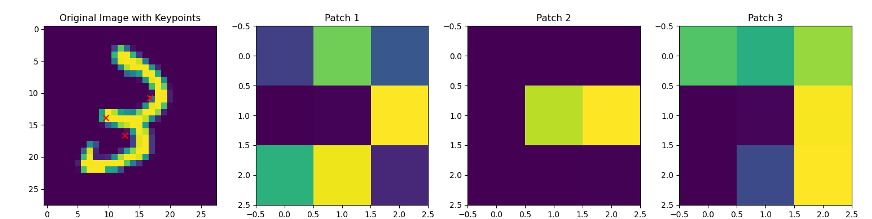
\includegraphics[scale=0.35]{images/Picture3.png}
    \caption{Here we can see that the focus-based model picked keypoints that are in the middle line of the 3 and the 2 coves. We can guess that the model is focusing on these features to classify the image.}
    \label{fig:focus-3}
\end{figure}

Similarly on Fashion-MNIST, the focus-based model was able to achieve a test accuracy of 86\% using \(\text{patch\_size} = 5\). This is a bit lower than the accuracy of a standard CNN for this problem but still comparable. Similarly, the model was able to achieve this accuracy with a much smaller number of parameters than a standard CNN.

However, on larger datasets such as CIFAR-10, the focus-based model was only able to achieve a test accuracy of 52\% using \(\text{patch\_size} = 5\). This is significantly lower than the accuracy of a standard CNN, however, this can be mostly explained by the fact that the model is much smaller than a standard CNN.



\subsection{Corner-based model results:}
The corner-based model lagged behind the focus-based model in accuracy, achieving a test accuracy of 86\% on MNIST and 72\% on Fashion-MNIST. This is likely due to the fact that the corner detection algorithm is not as complex as the focus model and corners are not a perfect heuristic for finding keypoints. The corner detection algorithm only scored 34\% on CIFAR-10, which is significantly lower than the focus-based model. These more complex datasets require more complex models to achieve high accuracy.

\begin{figure}[hbt!]
    \centering
    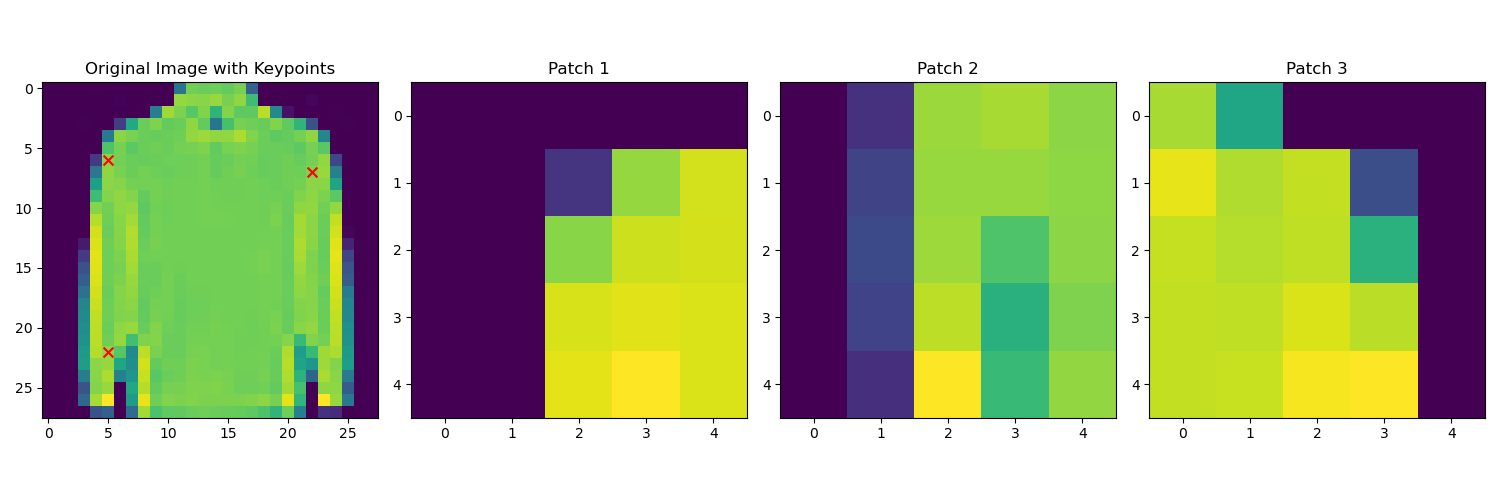
\includegraphics[scale=0.20]{images/corner_on_FashionMNIST.png}
    \caption{Here we can see that corner-based model picked keypoints that are in the connection between the sleaves and the body of the shirt.}
    \label{fig:focus-3}
\end{figure}

\section{Attention-based model results:} The attention-based CNN model was comparable in both accuracy and efficiency to its generic CNN counterpart. However, this model stood out in explainability. The attention maps extracted from the CNN allowed for enhanced interpretability visualized aggregated information in the important layers of the CNN. These attention maps are also directly factored into the decision of the model, making there some level of consistency in the visuals in and the decision.
\begin{figure}[hbt!]
    \centering
    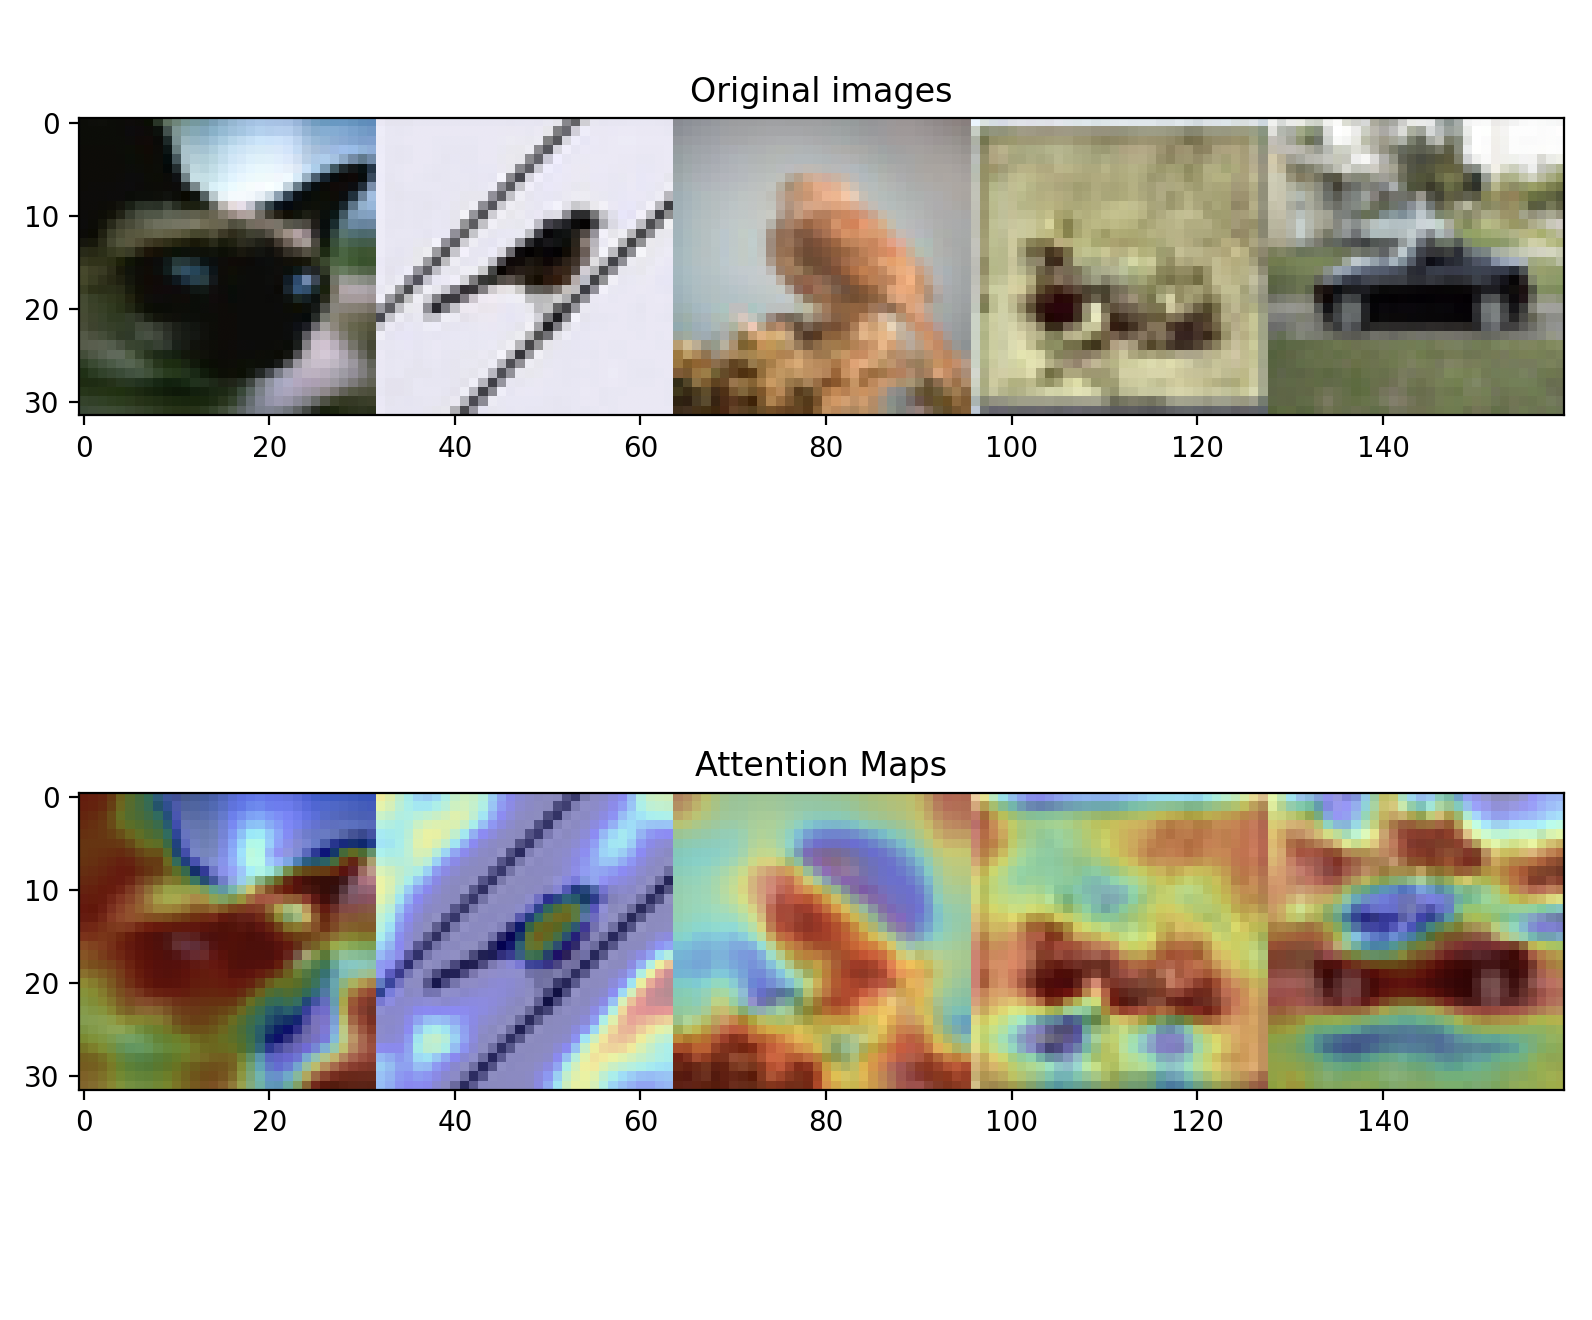
\includegraphics[width=\linewidth]{images/attentionheatmap.png}
    \caption{Attention maps overlaid on classified images}
    \label{fig:result1}
\end{figure}

\begin{figure}[hbt!]
    \centering
    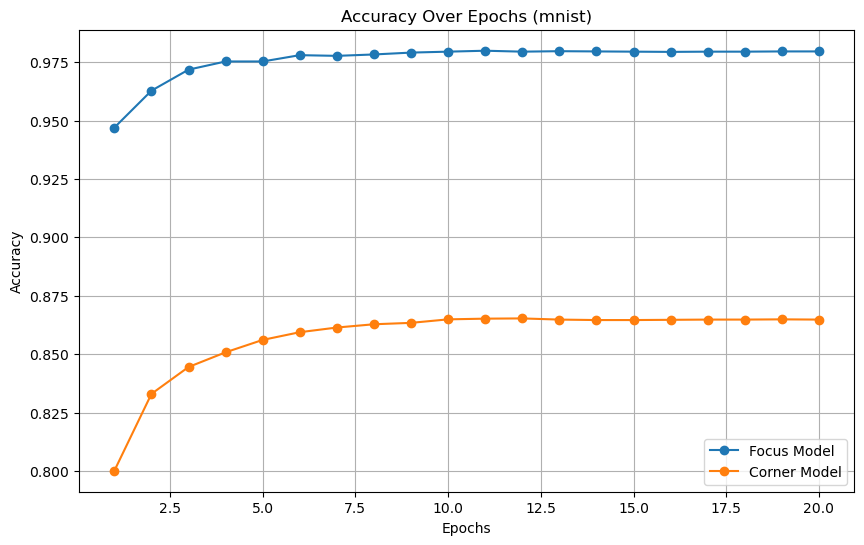
\includegraphics[width=\linewidth]{images/mnist.png}
    \caption{Accuracy on MNIST}
    \label{fig:mnist}
\end{figure}
\begin{figure}[hbt!]
    \centering
    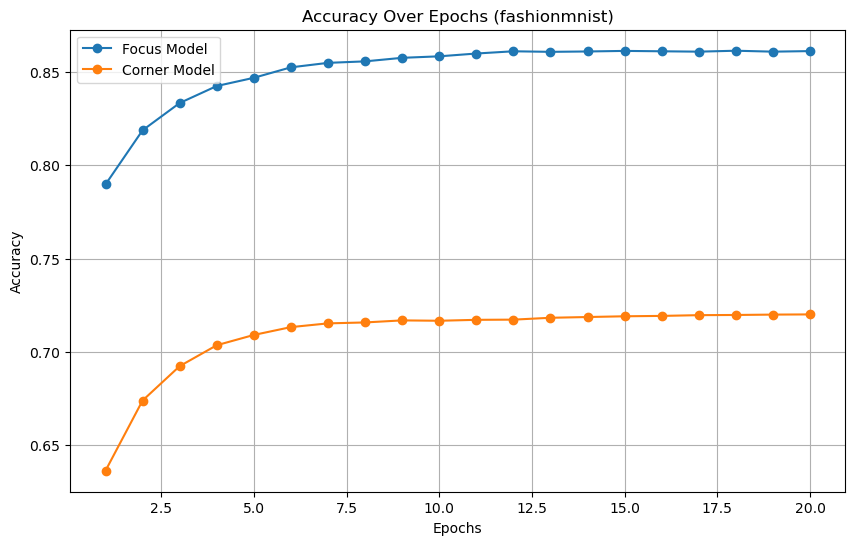
\includegraphics[width=\linewidth]{images/fashion.png}
    \caption{Accuracy on FashionMNIST}
    \label{fig:fashion}
\end{figure}
\begin{figure}[hbt!]
    \centering
    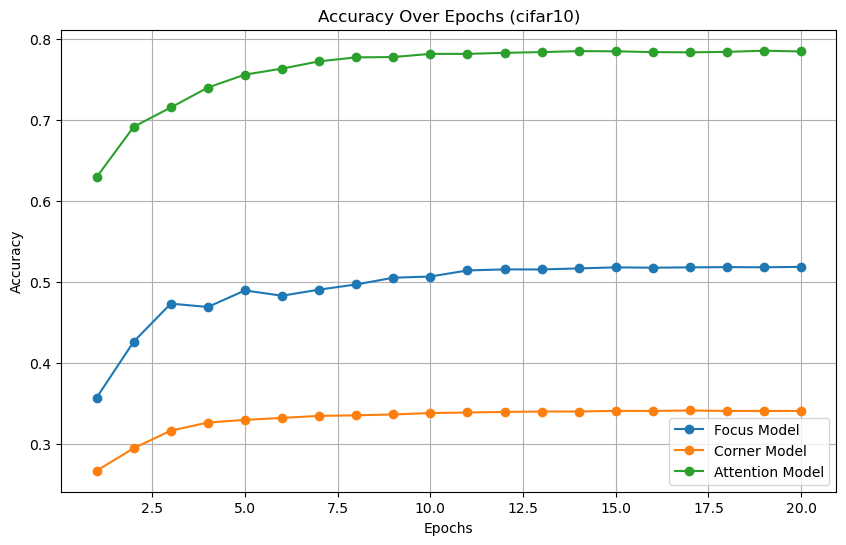
\includegraphics[width=\linewidth]{images/cifar.png}
    \caption{Accuracy on CIFAR10}
    \label{fig:cifar}
\end{figure}

%-------------------------------------------------------------------------
\subsection{Technical Discussion}

In attempting to increase CNN image classification efficiency and explainability while maintaining accuracy comparable to that of a traditional CNN, our method raises the question of the extent to which model efficiency, accuracy, and explainability are related. For instance, in the highly efficiency corner focus-based CNN, we observe that as image complexity increased, the models accuracy decreased, as seen in its accurate performance on the MNIST and Fashion MNIST datasets compared to its inaccurate performance on the CIRFAR dataset. In this instance, high efficiency in the model led to a compromise of its accuracy, highlighting the tradeoff of efficiency for accuracy as image complexity increases. This leads to the question of whether creating a model which can score highly across accuracy, efficiency and explainability while remaining generalizable to images of varying complexity is possible. Additionally, our method results highlights that our saliency models led to increased performance efficiency whereas our attention model increased accuracy and explainability but led to a tradeoff of increased computation time. To these ends, our methods and results highlight certain relationships and tradeoffs between model efficiency, explainability, and accuracy in image classification. Moreover, regardless of the tradeoffs, the changes made to our model by adopting saliency and attention techniques led to increased explainability. 


%------------------------------------------------------------------------
\section{SRC Discussion and Critique}

% The techniques we explored to increase image classification efficiency and explainability in a CNN and the results raises could have a few societal implications. With regards to biometric authentication in passwords, if a company decides to increase algorithm efficiency, this could compromise accuracy and thus compromise the devices security. Furthermore, biometric passwords are commonplace in our world today, and therefore overly prioritizing the algorithm's efficiency could seriously decrease the security of many people's personal information ultimately leading to a less secure world. Additionally, our models increased explainability could have positive impacts in the field of medicine, as image processing in diagnosis may have more explainable, and thus reliable results, leading to greater confidence in diagnosis, making them safer to implement in hospitals. 

In the interest of brevity, we've shortened sections of the critique (in italics) and responded to each section independently.

\emph{While there may be benefits for patients in medical image classification applications, one criticism is that the explainability may not be comprehensible by a normal person including patients...it may introduce more confusion than understanding.}

Although this might be true, especially in a medical setting, our hope was this method made it directly clear what sections were important to the model by embedding the explainability components directly into the model rather than a hindsight perspective using LIME. Some of the results may still be needed to be explained by an expert but it can also help point out where to look with both using keypoint and attention. For example, the saliency-based models could find something that could look like a tumor and then use the classification model to confirm and provide an overall classification. A doctor could step in between the two models to observe the keypoints that the saliency based model focused on.

\emph{Another critique is that the model won’t be successful for medical imaging if a new piece of data is encountered.}

This is true for our model as well as any model, and maybe more importantly with experts too. This is why our lawyers read so many cases, our doctors spend so much time in residency, and our teachers are sometimes graded on how long they've been teaching. Our experts are experts because of their experience and have trained on lot of data in order to optimally complete the task no matter what they are given. All we can really prepare for this is by making sure our training data reflects the real world i.e. our data lacks any major bias. And it is true that there is some blame to go around if a model that is supposed to be used on a particular distribution of data is used on another, leading to misclassifications.

\emph{Another stakeholder to consider is doctors who will use this technology and how they will assume responsibility for any false negatives and false positives that happen in the process.}

This is a valid concern and in life-threatening situations the model should be used as an addition or guide rather than a replacement for an expert. Moreover, our model might be able to help more with this than other models since it shows more about what details it considered for the result, so the expert can "consult" the model by seeing what the model is focusing on and then come up with their own decision like in the previous example with a cancer diagnosis. This would ensure that the expert + model pair can be strictly more accurate than just the expert.

\emph{The proposal suggested that once this technology is implemented, websites that use CAPTCHA are in danger of being spammed by bots. However, most CAPTCHA tests are not solely looking at the classification accuracy but rather look at the browsing history and how fast the user has clicked on a hyperlink.}

This is is referring to relatively new CAPTCHAs. The old CAPTCHAs still uses image classification with bounding boxes. And when the new CAPTCHAs fail, they fall back on the old CAPTCHAs. Some websites still use the old CAPTCHAs and whenever you use a CAPTCHA after you clear any cookies and site browsing data it will ussally fail back on the old CAPTCHAs. So this concern can still be relevent - some of the saliency based methods could inspire more efficient models that malicious actors can use to subvert CAPTCHAs. 
\section{Conclusion}

% What you did, why it matters, what the impact is going forward.
In this project, we explored ways to adopt human-based visual processing in a convolutional neural network (CNN) in order to create a model which classifies images with greater efficiency and explainability compared to that of a traditional CNN while maintaining a comparable accuracy. Furthermore, we strove to achieve this by utilizing a saliency-based CNN, which made use of two separate methods, being focus and corner detection, as well as an attention-based CNN. With the saliency-based CNN, we were able to increase computation efficiency and provided a level of explainability while maintaining comparable accuracy to a traditional CNN on the MNIST and fashion MNIST datasets. However, this efficiency was a tradeoff for accuracy on datasets containing more detailed images such as CIRFAR. The attention model demonstrated a much higher accuracy relative to the saliency-based approaches and provided a layer of explainability, but this compromised efficiency as there was a much longer computation time. These results highlight the potential tradeoffs between model efficiency, explainability, and accuracy with respect to image detail and complexity in CNN image classification. Furthermore, these results highlight that society, stakeholders should be careful when optimizing for efficiency not to compromise accuracy when using these tools, as this could lead to severe compromises, namely in security and medicine, as explored in section seven. 


{\small
\bibliographystyle{plain}
\bibliography{report}
}

\section*{Appendix}

\subsection*{Team contributions}

Please describe in one paragraph per team member what each of you contributed to the project.
\begin{description}
\item[Siddu Sitaraman]
This team member contributed through working on the implementation of the attention model and fronting much of the research into attention in the paper. Additionally, this team member worked to get OSCAR working for the models and contributed technical help with the other team members.
\item[George Chemmala]
This team member contributed through working on the implementation of the focus model and setting up the general saliency model. Additionally, this team member, along with the previous team member, worked to get OSCAR working for the models and managed much of the development practices.
\item[Triston Roberts] 
This team member contributed through working on the implementation of the corner detection based CNN by utilizing harris corner detection as discussed in section 4.1.2. Additionally, this team member researched various saliency methods to incorporate into the CNN model, and contributed to the poster and its format, as well as writing various sections on the final report. 
\end{description}

\end{document}
